\documentclass[,jou, a4paper,floatsintext]{apa6}
\usepackage{lmodern}
\usepackage{amssymb,amsmath}
\usepackage{ifxetex,ifluatex}
\usepackage{fixltx2e} % provides \textsubscript
\ifnum 0\ifxetex 1\fi\ifluatex 1\fi=0 % if pdftex
  \usepackage[T1]{fontenc}
  \usepackage[utf8]{inputenc}
\else % if luatex or xelatex
  \ifxetex
    \usepackage{mathspec}
  \else
    \usepackage{fontspec}
  \fi
  \defaultfontfeatures{Ligatures=TeX,Scale=MatchLowercase}
\fi
% use upquote if available, for straight quotes in verbatim environments
\IfFileExists{upquote.sty}{\usepackage{upquote}}{}
% use microtype if available
\IfFileExists{microtype.sty}{%
\usepackage{microtype}
\UseMicrotypeSet[protrusion]{basicmath} % disable protrusion for tt fonts
}{}
\usepackage{hyperref}
\hypersetup{unicode=true,
            pdftitle={Researchers Decision to Sign is Related to Their Recommendation},
            pdfauthor={Nino van Sambeek~\& Daniël Lakens},
            pdfkeywords={Peer Review, Open Science, Transparency},
            pdfborder={0 0 0},
            breaklinks=true}
\urlstyle{same}  % don't use monospace font for urls
\usepackage{graphicx,grffile}
\makeatletter
\def\maxwidth{\ifdim\Gin@nat@width>\linewidth\linewidth\else\Gin@nat@width\fi}
\def\maxheight{\ifdim\Gin@nat@height>\textheight\textheight\else\Gin@nat@height\fi}
\makeatother
% Scale images if necessary, so that they will not overflow the page
% margins by default, and it is still possible to overwrite the defaults
% using explicit options in \includegraphics[width, height, ...]{}
\setkeys{Gin}{width=\maxwidth,height=\maxheight,keepaspectratio}
\IfFileExists{parskip.sty}{%
\usepackage{parskip}
}{% else
\setlength{\parindent}{0pt}
\setlength{\parskip}{6pt plus 2pt minus 1pt}
}
\setlength{\emergencystretch}{3em}  % prevent overfull lines
\providecommand{\tightlist}{%
  \setlength{\itemsep}{0pt}\setlength{\parskip}{0pt}}
\setcounter{secnumdepth}{0}
% Redefines (sub)paragraphs to behave more like sections
\ifx\paragraph\undefined\else
\let\oldparagraph\paragraph
\renewcommand{\paragraph}[1]{\oldparagraph{#1}\mbox{}}
\fi
\ifx\subparagraph\undefined\else
\let\oldsubparagraph\subparagraph
\renewcommand{\subparagraph}[1]{\oldsubparagraph{#1}\mbox{}}
\fi

%%% Use protect on footnotes to avoid problems with footnotes in titles
\let\rmarkdownfootnote\footnote%
\def\footnote{\protect\rmarkdownfootnote}


  \title{Researchers Decision to Sign is Related to Their Recommendation}
    \author{Nino van Sambeek\textsuperscript{1}~\& Daniël Lakens\textsuperscript{1}}
    \date{}
  
\shorttitle{Recommendation Relates to Signing}
\affiliation{
\vspace{0.5cm}
\textsuperscript{1} Eindhoven University of Technology, The Netherlands}
\keywords{Peer Review, Open Science, Transparency\newline\indent Word count: 4926}
\usepackage{csquotes}
\usepackage{upgreek}
\captionsetup{font=singlespacing,justification=justified}

\usepackage{longtable}
\usepackage{lscape}
\usepackage{multirow}
\usepackage{tabularx}
\usepackage[flushleft]{threeparttable}
\usepackage{threeparttablex}

\newenvironment{lltable}{\begin{landscape}\begin{center}\begin{ThreePartTable}}{\end{ThreePartTable}\end{center}\end{landscape}}

\makeatletter
\newcommand\LastLTentrywidth{1em}
\newlength\longtablewidth
\setlength{\longtablewidth}{1in}
\newcommand{\getlongtablewidth}{\begingroup \ifcsname LT@\roman{LT@tables}\endcsname \global\longtablewidth=0pt \renewcommand{\LT@entry}[2]{\global\advance\longtablewidth by ##2\relax\gdef\LastLTentrywidth{##2}}\@nameuse{LT@\roman{LT@tables}} \fi \endgroup}

\authornote{This work was supported by the Netherlands Organization for Scientific Research (NWO) VIDI grant 452-17-013.

Correspondence concerning this article should be addressed to Daniël Lakens, ATLAS 9.402, 5600 MB, Eindhoven, The Netherlands. E-mail: \href{mailto:D.Lakens@tue.nl}{\nolinkurl{D.Lakens@tue.nl}}}

\abstract{
Open review is becoming increasingly common. Surveys indicate that researchers are generally positive about making peer reviews available. Researchers are more negative about revealing the identity of reviewers. In part this is because of the possibility that reviewers will be less likely to express criticisms if their identity is known to authors. Experiments suggest that reviewers might be somewhat more likely to recommend to accept articles when they are told their name will be shared alongside the reviews, than when they will remain anonymous. So far, there is surprisingly little information about what reviewers actually do in practice. We analyzed XXXX open reviews in PeerJ and XXXX reviews in the Royal Society Open Science and Open Biology to examine whether in practice the propability that a reviewer reveals their identity is related to their recommendation. When comparing XXXX signed and XXXX unsigned reviews, we observed a clear pattern where the more positive a recommendation, the more likely it was signed. Although our data does not allow for inferences about causal relationships, it provides behavioral data from real peer reviews that demonstrates convincingly that reviewers who sign their reviews give more positive recommendations.


}

\begin{document}
\maketitle

As technology advances, science advances. The rise of the internet has made it possible to share all aspects of the scientific process. This includes opening up the peer review process. An increasing number of journals has started to make peer review reports available alongside published articles as part of ongoing experiments that aim to improve the peer review process (Bruce, Chauvin, Trinquart, Ravaud, \& Boutron, 2016). Having access to these peer review reports makes it possible to gain new insights about how scientists perform reviews.

Some journals have chosen to not just share reviews publicly when an article is published, but in addition require reviewers to sign their reviews. An important argument for such a policy is that reviewers can receive credit for their work (Godlee, 2002). However, scientists do not feel these benefits outweigh possible costs. Researchers indicate they would be less likely to review for a journal if their names are made public, and anecdotally mention that signed reviews would make it more difficult to be honest about poor quaity papers (Mulligan, Hall, \& Raphael, 2013). A more recent survey among almost 3000 scientists found that 50.8\% of reviewers believe signed open reviews would make peer review worse (Ross-Hellauer, Deppe, \& Schmidt, 2017). Almost two-thirds of respondents believed reviewers would be less likely to deliver strong criticisms if their identity became known to the authors.

These self-report studies are complemented by experiments in which reviewers are been randomly assigned to a condition where their names would be added to their reviews or not (Walsh, Rooney, Appleby, \& Wilkinson, 2000). Reviewers in the signed condition were less likely to recommend rejection (n = 30) than researchers in the unsigned condition (n = 51). This suggests that a causal effect exists between knowing your name will be known or not and the recommendation reviewers provide. Across four studies, a meta-analysis by Bruce and colleagues (2016) supports the conclusion that reviewers are somewhat less likely to recommend rejection when they have to sign their reviews.

Although the self-report studies and the experiments clearly suggest reviewers worry about having their name attached to highly critical reviews, so far little is known about what reviewers actually do when given the opportunity to sign their reviews. The trade-off between the benefit of getting credit for peer review work and the risk of negative consequences when signing critical reviews might lead to strategic behavior where authors become more likely to sign reviews the most positive their recommendation is. If this strategic behavior occurs in practice, we should see a different pattern of recommendations for signed and unsigned reviews. One recent study revealed such a pattern when analyzing data from an Elsevier trial on publishing peer review reports in the journal Agricultural and Forest Meteorology, Annals of Medicine and Surgery, Engineering Fracture Mechanics, Journal of Hydrology: Regional Studies, and the International Journal of Surgery (Bravo, Grimaldo, López-Iñesta, Mehmani, \& Squazzoni, 2019). Although only 8.1\% of reviewers choose to disclose their identity in these reviews, but the data revealed a clear difference between the recommendations by reviewers who chose to sign their reviews, compared to reviewers who did not choose to sign. Here, we examine this pattern in two large open access journals that publish across a wide range of scientific disciplines. In this replication and extension of the analysis by Bravo and colleagues (2019) we examine the relationship between recommendations and signed reviews in open peer reviews in mega-journals that publish scientific work across a wide range of scientific disciplines.

\hypertarget{accessing-open-peer-reviews}{%
\section{Accessing Open Peer Reviews}\label{accessing-open-peer-reviews}}

To examine the pattern of recommendations as a function of whether reviewers signed their review or not we analyzed 3576 articles published in The Royal Society Open Science and Open Biology, and 7223 articles published in PeerJ. PeerJ launched in 2012 and gave reviewers the possibility to sign, and authors to make the peer reviews available with the final publication. The Royal Society Open science launched in 2014 and strongly encouraged authors to make the peer reviews available with the final publication. Royal Society Open Biology made sharing reviews with the final publication mandatory in 2017. Because of their broad scope, the large number of publications in each journal, and their early focus on open reviews, these reviews provide insights into the peer review behavior of scientists across a wide range of disciplines.

PeerJ assigns all articles a number, increasing consecutively with each published manuscript. Reviews are always accessible in html (i.e., at \url{https://peerj.com/articles/1/reviews} for the first article can be found). Reviews of articles published in The Royal Society Open Science and Open Biology are published online with the articles as PDF files. A list of Digital Object Identifiers (DOIs) for every article published in these two outlets was retrieved through Scopus. All reviews were downloaded, and the PDF files were exported to plain text files using pdftools (Ooms, 2019). These text files were mined for recommendations, reviewers names, submission and acceptance dates, and the review content, using the stringr package (Wickham, 2019).

For each article we extracted the number of revisions, and for each revision we saved for each review whether the reviewer signed or not, the word count for their review, and the recommendation for that review round. Note that for PeerJ recommendations each round are giving by the editor. We therefore do not directly know which recommendation each reviewer provided, but analyze the data based on the assumption that the decision by the editor is correlated with the underlying reviews. For RSOS and RSOB reviewers do recommend to \enquote{accept as is}, \enquote{accept with minor revisions}, \enquote{major revision}, or \enquote{reject}. Although \enquote{reject} recommendations occur for RSOS and RSOB, both PeerJ and RSOS and RSOB only share reviews for published articles, and therefore we have very few reject recommendation in RSOS and RSOB, and none in PeerJ. Searching all reviews for PeerJ for the words \enquote{appealed on} reveals 44 articles that were initially rejected, appealed, received a \enquote{major revision} recommendation, and were eventually published. We have coded these papers as \enquote{major revisions}. All scripts to download and analyze the reviews, and computationally reproduce this manuscript, are available at \url{https://osf.io/jkbmw/}.

\hypertarget{peer-review-reports}{%
\section{Peer Review Reports}\label{peer-review-reports}}

PeerJ provides authors the option to publish the peer reviews of their article alongside the final publication of the article. The Royal Society Open Science and Open Biology also provided authors with the option to publish peer reviews alongside the article, and made this mandatory from May 2017 (Open Biology) and January 2019 (Open Science). Peer reviewers have the option to provide their names to the authors when submitting their peer review for both PeerJ and Royal Society Open Science and Open Biology.

We examined the first 7223 articles pubished in PeerJ, as well as the first 2887 articles in RSOS and the first 689 articles in RSOB. We retrieved all reviews for all review rounds of 4555 articles in PeerJ, 1412 articles in RSOS, and 148 articles in RSOB. Articles can go through multiple rounds of review. We focus on the first review round as this review reflects the initial evaluation of reviewers, before the handling editor has made a decision, following (Bravo et al., 2019). On average initial submissions at PeerJ received 2.36 reviews. Articles in the Royal Society journals received on average 2.19 reviews for the original submission.

\hypertarget{signed-reviews-as-a-function-of-the-recommendation}{%
\section{Signed reviews as a function of the recommendation}\label{signed-reviews-as-a-function-of-the-recommendation}}

When analyzing all reviews of original submissions in PeerJ 4172 reviewers signed their reviews and 6569 did not. In The Royal Society journals 1261 reviewers signed their first review while 2150 did not. The percentages of people who sign (38.84\% for PeerJ, 36.97\% for the Royal Society) are slightly lower than the 43.23\% reported by (Wang, You, Manasa, \& Wolfram, 2016), who analyzed the first 1214 articles published in PeerJ.

To answer our main research question we plotted the signed an unsigned reviews as a function of the recommendation in the first review round. Remember that for PeerJ these recommendations are made by the editor, and thus only indirectly capture the evaluation of the reviewer. The percentage of signed peer reviews is larger for minor revisions (46.37\%) than it is for major revisions (34.63\%). Too few articles are accepted after the initial revision in PeerJ (20 in total) to provide reliable estimates for this category.

\begin{figure}
\centering
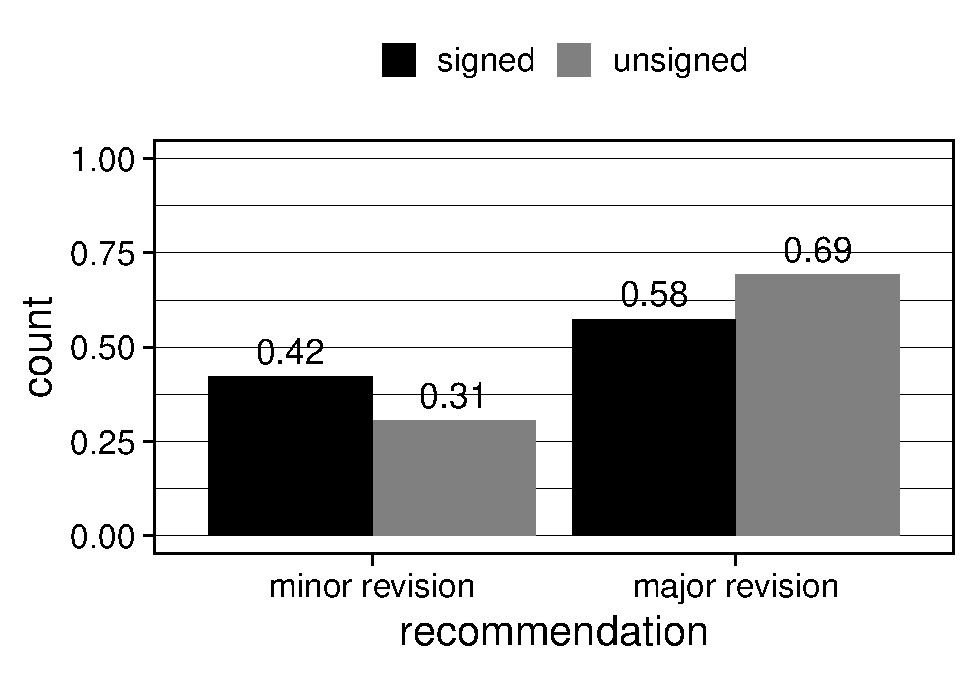
\includegraphics{open_peer_review_files/figure-latex/PeerJrec-1.pdf}
\caption{\label{fig:PeerJrec}Frequencies of signed and unsigned reviews as a function of whether the handling editor at PeerJ recommended \enquote{minor revisions} or \enquote{major revisions}.}
\end{figure}

Analyzing the reviews at the Royal Society provides a more direct answer to our question, since each individual reviewer is asked to provide a recommendation of \enquote{accept}, \enquote{minor revisions}, \enquote{major revisions}, or \enquote{reject}. We can therefore directly compare how recommendations are related to the decision to sign reviews. The percentage of signed peer reviews is decreases as recommendations become more negative, from 46.99\% for \enquote{accept} recommendations, 43.86\% for \enquote{minor revisions}, 29.48\% for \enquote{major revisions}, and 11.07\% for \enquote{reject} recommendations.

\begin{figure}
\centering
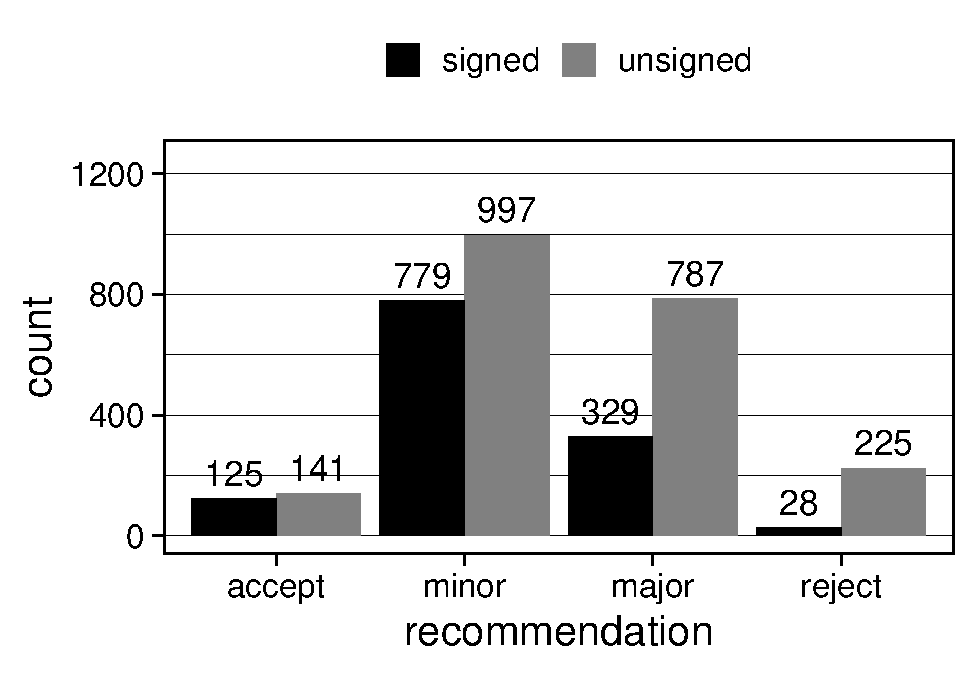
\includegraphics{open_peer_review_files/figure-latex/TRSrec-1.pdf}
\caption{\label{fig:TRSrec}Frequencies of signed and unsigned reviews as a function of whether the reviewer at the Royal Society Open Science and Open Biology recommended \enquote{accept}, \enquote{minor revisions}, \enquote{major revisions}, or \enquote{reject}.}
\end{figure}

Since these data are correlational we can not draw causal conclusions. It is possible that reviewers are less likely to sign more negative reviews. It is also possible that people who sign their reviews are in general less negative in their recommendations, and therefore the distribution of signed reviews differs from non-signed reviews. Given the literature described in the introduction that provides anecdotal evidence researchers worry they will be able to provide open criticism if their names are public, and experimental evidence suggesting that if names are made public, recommendation become somewhat more positive, it seems plausible at least part of the pattern we observed can be explained by reviewers being more likely to sign their more positive reviews. Our results replicate the observations by Bravo and colleagues (2019).

\hypertarget{additional-analyses}{%
\section{Additional Analyses}\label{additional-analyses}}

The dataset we are sharing has information about the recommendations of reviewers or editors after each round of peer review, the names of reviewers who signed their review, and the time in review (112 days for PeerJ, 133 days for RSOS and RSOB). Through the DOI, researchers can link this data to other sources of information such as citation counts. Because the reviews themselves are included in our dataset, researchers interested can use the text files to answer more details questions about the content of peer reviews across different domains. For example, we can examine the word count for signed and unsigned reviews as a function of the recommendation. With the caveat that the graph below present uncleaned raw word counts, we replicate the results reported by (Wang et al. (2016)) for PeerJ in the dataset for Royal Society Open Science and Open Biology that there is no statistical difference between the word count for signed and unsigned reviews, despite a small numerical difference in the same direction as in their analysis of PeerJ reviews.

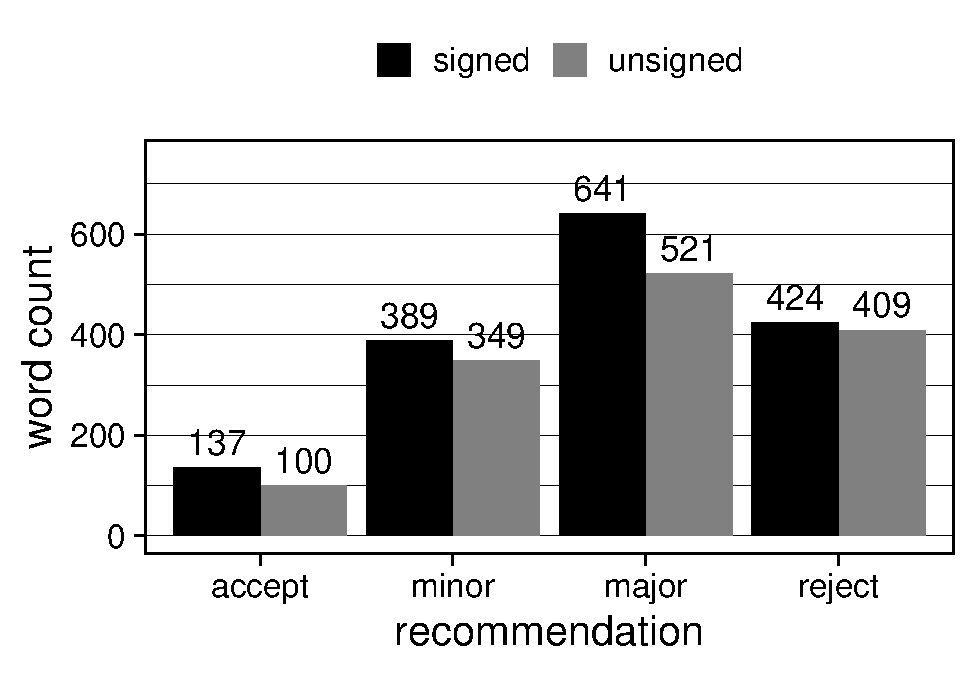
\includegraphics{open_peer_review_files/figure-latex/wordcount-1.pdf}

Since multiple reviewers for The Royal Society Open Science and Open Biology make their individual recommendations known, one example of the insights open reviews provide is how often reviewers agree. For the 1559 individual papers that we were able to retrieve reviews from, reviewers agreed on the recommendation in 646 (41.44\%) of the time. For 42.14\% of the manuscripts the maximum deviation was one category (e.g., minor and major revisions), for 14.69\% of the manuscripts the maximum deviation was two categories (e.g., accept and major revision), and for 1.73\% of the manuscripts the maximum deviation was three categories (i.e., accept and reject). There were 3 articles where researchers received all four possible recommendations (accept, minor revisions, major revisions, reject) from at least four different reviewers.

Regrettably, neither PeerJ nor RSOS make peer reviews available for manuscripts that were rejected. As a consequence, we have analyzed a biased sample of the literature. At the moment only very few scientific journals (e.g., Meta-Psychology, F1000) make peer reviews available for all submitted articles. Although open reviews enable us to look in more detail at the peer review process, it would be extremely interesting to be able to follow manuscripts through the peer review process even when they are rejected at specific journals. Despite this limitation, the pattern of results is very similar to that observed by Bravo and colleagues (2019) who had access to the reviews for accepted and rejected manuscripts. Thus, even though the proportion of reject recommendation in our dataset is small, the relative difference with which this recommendation is given in signed and unsigned reviews seems comparable to datsets that include rejected manuscripts.

\hypertarget{discussion}{%
\section{Discussion}\label{discussion}}

Our analysis shows that when authors are given the choice to sign their reviews, signed reviews have more positive recommendations than unsigned reviews. This is true for reviews in Royal Society Open Science, a large multi-disciplinary journal that published across a wide range of scientific domains. The effect is also visible in a second large multi-disciplinary journal, PeerJ, under the assumption that recommendations by editors at PeerJ are correlated with the recommendations by reviewers. Our results replicate and extend earlier findings by Bravo et al. (2019), and complement self-report and experimental results. Although our results do not allow for causal claims, they are in line with experimental results that reveal researchers give more positive recommendations when their name is published alongside their reviews (Bruce et al., 2016).

Open reviews allow researchers to adress meta-scientific questions that give insights into the peer review process. Our data provide further support for the idea that researchers decision to sign is related to their recommendation across a wide range of scientific disciplines. Our correlational data, interpreted together with self-report data and experiments in the literature, increases the plausibility that in real peer reviews at least some researchers are more likely to sign if their recommendation is more positive. This type of strategic behavior also follows from a purely rational strategy to optimize the benefits of peer review while minimizing the costs. For positive recommendations, reviewers will get credit for theor reviews, while for negative reviews, they do not run the risk of receiving any backlash from collegaues in their field.

It is worthwhile to examine whether this fear of retaliation has an empirical basis, and if so, to consider developing guidelines to counteract such retaliation (Bastian, 2018). Althoughit looks increasingly plausible that at least some reviewers feel hesitant to sign if they believe doing so could have negative consequences, but are willing to sign to gain credit for their work for more positive recommendations, it seems wortwhile to explore ways in which they can receive credit for all their peer review work, also when their recommendations are more negative. If more journals share open reviews, also for rejected manuscripts, future meta-scientific work might be able to study this important topic in more detail.

\hypertarget{author-contributions}{%
\section{Author Contributions}\label{author-contributions}}

N. van Sambeek and D. Lakens developed the idea, and jointly created the R code to generate and analyze the data. N van Sambeek drafted the initial version of the manuscript as a Bachelor thesis, D. Lakens drafted the final version, and both authors revised the final version of the manuscript.

\hypertarget{conflict-of-interest-statement}{%
\section{Conflict of Interest Statement}\label{conflict-of-interest-statement}}

The authors report no conflicts of interest.

\hypertarget{references}{%
\section{References}\label{references}}

\setlength{\parindent}{-0.5in}
\setlength{\leftskip}{0.5in}

\hypertarget{refs}{}
\leavevmode\hypertarget{ref-bastian_signing_2018}{}%
Bastian, H. (2018). Signing Critical Peer Reviews \& the Fear of Retaliation: What Should We Do? \textbar{} Absolutely Maybe. https://blogs.plos.org/absolutely-maybe/2018/03/22/signing-critical-peer-reviews-the-fear-of-retaliation-what-should-we-do/.

\leavevmode\hypertarget{ref-bravo_effect_2019}{}%
Bravo, G., Grimaldo, F., López-Iñesta, E., Mehmani, B., \& Squazzoni, F. (2019). The effect of publishing peer review reports on referee behavior in five scholarly journals. \emph{Nature Communications}, \emph{10}(1), 1--8. doi:\href{https://doi.org/10.1038/s41467-018-08250-2}{10.1038/s41467-018-08250-2}

\leavevmode\hypertarget{ref-bruce_impact_2016}{}%
Bruce, R., Chauvin, A., Trinquart, L., Ravaud, P., \& Boutron, I. (2016). Impact of interventions to improve the quality of peer review of biomedical journals: A systematic review and meta-analysis. \emph{BMC Medicine}, \emph{14}. doi:\href{https://doi.org/10.1186/s12916-016-0631-5}{10.1186/s12916-016-0631-5}

\leavevmode\hypertarget{ref-godlee_making_2002}{}%
Godlee, F. (2002). Making Reviewers Visible: Openness, Accountability, and Credit. \emph{JAMA}, \emph{287}(21), 2762--2765. doi:\href{https://doi.org/10.1001/jama.287.21.2762}{10.1001/jama.287.21.2762}

\leavevmode\hypertarget{ref-mulligan_peer_2013}{}%
Mulligan, A., Hall, L., \& Raphael, E. (2013). Peer review in a changing world: An international study measuring the attitudes of researchers. \emph{Journal of the American Society for Information Science and Technology}, \emph{64}(1), 132--161. doi:\href{https://doi.org/10.1002/asi.22798}{10.1002/asi.22798}

\leavevmode\hypertarget{ref-ooms_pdftools_2019}{}%
Ooms, J. (2019). \emph{Pdftools: Text extraction, rendering and converting of PDF documents}.

\leavevmode\hypertarget{ref-ross-hellauer_survey_2017}{}%
Ross-Hellauer, T., Deppe, A., \& Schmidt, B. (2017). Survey on open peer review: Attitudes and experience amongst editors, authors and reviewers. \emph{PLOS ONE}, \emph{12}(12), e0189311. doi:\href{https://doi.org/10.1371/journal.pone.0189311}{10.1371/journal.pone.0189311}

\leavevmode\hypertarget{ref-walsh_open_2000}{}%
Walsh, E., Rooney, M., Appleby, L., \& Wilkinson, G. (2000). Open peer review: A randomised controlled trial. \emph{The British Journal of Psychiatry}, \emph{176}(1), 47--51. doi:\href{https://doi.org/10.1192/bjp.176.1.47}{10.1192/bjp.176.1.47}

\leavevmode\hypertarget{ref-wang_open_2016}{}%
Wang, P., You, S., Manasa, R., \& Wolfram, D. (2016). Open peer review in scientific publishing: A Web mining study of PeerJ authors and reviewers. \emph{Journal of Data and Information Science}, \emph{1}(4), 60--80.

\leavevmode\hypertarget{ref-wickham_stringr_2019}{}%
Wickham, H. (2019). \emph{Stringr: Simple, consistent wrappers for common string operations}.


\end{document}
